\begin{center}
\Large\textbf{Language Ideas for Quantum Hardware Comprehension}
\end{center}

\large{From idea to practice... 
\\ 
\space

\begin{figure}[htbp]
    \centering
    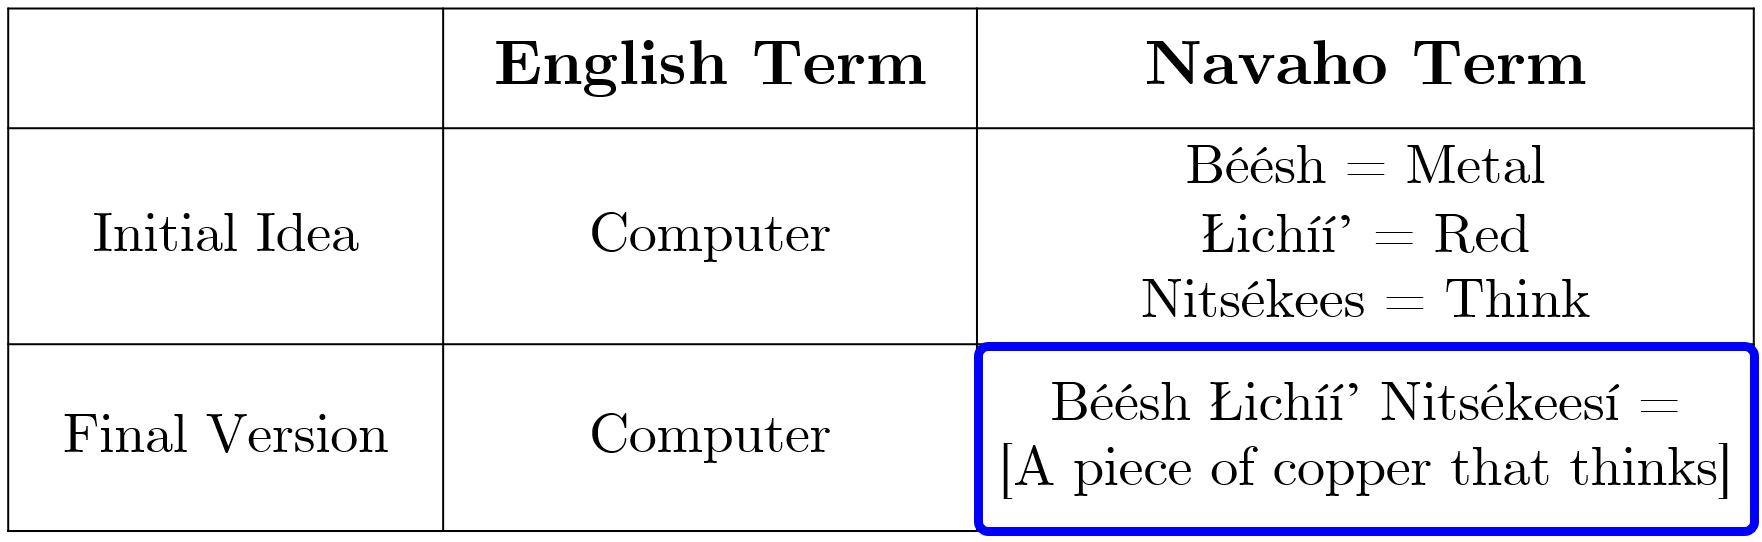
\includegraphics[width=0.9\textwidth]{Computer_NV.png}
    \caption{$Computer$ in Navaho.}
    \label{fig:svgImage}
\end{figure}
}

\large{
\noindent
Other examples:
\\ 
\space
\\
The quick brown fox = Ma'ii dibéłchíʼí tsį́įłgo or Ma'ii yishtłizh tsį́įłgo
\\
Lazy dog = léechąą’í iłhóyéé
\\
Jumped = nahachaʼ or dah nahachaʼ or dahnáníjįįh
\\
To jump = dahnáníshjį́į́h
\\
Jumping = dah nahácha’go
\\
Laziness = iłhóyéé
\\
Slow or in vain = chʼééh
\\
The quick brown fox jumped over the lazy dog = Ma'ii dibéłchíʼí tsį́įłgo léechąą’í iłhóyéé dahnáníjįįh
\space
}